\documentclass{beamer}
 
\usepackage[utf8]{inputenc}
\usepackage{amssymb,amsmath,amsthm, amsfonts}
\usepackage{mathrsfs}
\usepackage{kotex}
\usepackage{graphicx}
\usepackage{xcolor}
\usepackage{multimedia}
\usepackage{setspace}
\usepackage{multicol}
\usepackage{import}
\usepackage{color}
\usepackage{tikz} 
\usepackage{xcolor}
\usepackage{tkz-graph}
%\usepackage{minted}
\usepackage{listings}
\usetikzlibrary{arrows,shapes}
\graphicspath{{images/}}
\DeclareGraphicsExtensions{.pdf,.png,.jpg}

%%packages to make fixed-position textboxes
\usepackage[absolute,overlay]{textpos}
%\usepackage[texcoord,grid,gridcolor=red!10,subgridcolor=green!10,gridunit=pt]{eso-pic}

%% Color Setting %%
\definecolor{Grey}{rgb}{0.6,0.6,0.6}
\definecolor{NACred}{RGB}{105,0,0}
\definecolor{NACblue}{RGB}{70,70,170}
\definecolor{NACgrey}{RGB}{220,220,220}
\definecolor{GSHSRED}{RGB}{120,20,20}
\definecolor{GSHSBLUE}{RGB}{0,28,84}
\definecolor{gshsred}{RGB}{240,210,210}
\definecolor{gshsblue}{RGB}{240,240,250}
\definecolor{unistemerald}{RGB}{68,193,195}
\setbeamercolor{title}{bg=white,fg=NACblue}
\setbeamercolor{author}{fg=black}
\setbeamercolor{institute}{fg=GSHSBLUE}
\setbeamercolor{date}{fg=GSHSBLUE}
\setbeamercolor{logo}{bg=gshsblue}
\setbeamercolor{sidebar}{bg=GSHSRED}
\setbeamercolor{frametitle}{bg=GSHSBLUE,fg=white}
\setbeamercolor{section in sidebar}{use=sidebar,bg=white,fg=sidebar.bg}
\setbeamercolor{subsection in sidebar}{parent=section in sidebar}
\setbeamercolor{subsubsection in sidebar}{parent=subsection in sidebar}
\setbeamercolor{item}{fg=NACred}
\setbeamercolor{block title}{bg=unistemerald,fg=black}
\setbeamercolor{block body}{bg=gshsblue,fg=black}


\title[About Beamer] %optional
{매트로이드와 그리디 알고리즘}
 
\subtitle{Matroids and Greedy Algorithms}
 
\author[] % (optional, for multiple authors)
{Jongseo Lee}

%% Title Page Setting %%
\setbeamerfont{title}{}
\setbeamertemplate{title page}{
  %% Background Logo
  \begin{picture}(0,0)%
    \setlength{\unitlength}{1cm}% default
  \end{picture}%
  \vfill
  \vspace*{10mm}
  \centering
  %% Title
  \usebeamerfont{title}\usebeamercolor[fg]{title}\inserttitle\par
  \vskip 2mm
  %% Subtitle
  \ifx\insertsubtitle\@empty
  \else\usebeamerfont{subtitle}\usebeamercolor[fg]{subtitle}\insertsubtitle
  \fi

  \vskip 3mm
  %% Horizontal line
  \usebeamercolor[fg]{title}\hrule height 2pt\hfill
  \vskip 10mm
  %% Author
  \usebeamercolor[fg]{author}\usebeamerfont{author}\insertauthor
  \vskip 1cm
  %% Institute
  \usebeamercolor[fg]{institute}\usebeamerfont{institute}\insertinstitute
  \vskip 1cm
  %% Date
  \usebeamercolor[fg]{date}\usebeamerfont{date}\insertdate
  \vfill
}

%\institute[VFU] % (optional)
%{
%  \inst{1}%
%  Faculty of Physics\\
%  Very Famous University
%  \and
%  \inst{2}%
%  Faculty of Chemistry\\
%  Very Famous University
%}

\newcommand{\I}{\mathcal{I}}
\newcommand{\B}{\mathcal{B}}
\newcommand{\F}{\mathbb{F}}

\date[TWC 2019] % (optional)
{KAIST 수학문제연구회 $\mathcal{M}^2$\\KAIST School of Freshman\\November 18, 2019}
 
%\logo{\includegraphics[height=1.8cm]{nacom.png}}

%% itemize bullet setting %%
\setbeamertemplate{itemize items}[ball]

%% block setting %%
\setbeamertemplate{blocks}[rounded][shadow=true]
\addtobeamertemplate{block begin}{%
  \setlength{\textwidth}{300pt}%
}{}

%\addtobeamertemplate{frame}{\setlength\abovedisplayskip{0pt}}
%\setbeamerfont{frametitle}{size=\normalsize}

%% caption setting %%
\setbeamertemplate{caption}[numbered]
 \newenvironment{cpp}
  {\VerbatimEnvironment
   \begin{minted}[frame=lines]{c++}}
  {\end{minted}}
\begin{document}
\begin{frame}[plain]
\titlepage
\end{frame}

\begin{frame}[t]
{Today's Topic}

\begin{itemize}
    \item<1-> What is a matroid?
    \item<2-> Greedy algorithms
\end{itemize}

\end{frame}

\begin{frame}[t]
{Preliminaries}
Let $G = (V, E)$ be a graph.
\begin{center}
    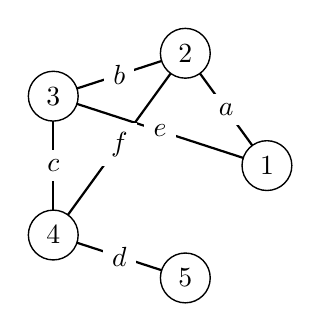
\begin{tikzpicture}
        %\GraphInit[vstyle=Welsh]
        \SetGraphUnit{1.5}
        \Vertices{circle}{1, 2, 3, 4, 5}
        \Edges[label=$a$](1, 2)
        \Edges[label=$b$](2, 3)
        \Edges[label=$c$](3, 4)
        \Edges[label=$d$](4, 5)
        \Edges[label=$e$](1, 3)
        \Edges[label=$f$](2, 4)
    \end{tikzpicture}
\end{center}
\end{frame}

\begin{frame}[t]
{Preliminaries}
Let $G = (V, E)$ be a graph.
\begin{itemize}
    \item Cycle
\end{itemize}
\only<1>{
\begin{center}
    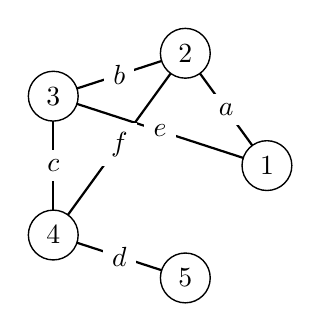
\begin{tikzpicture}
        %\GraphInit[vstyle=Welsh]
        \SetGraphUnit{1.5}
        \Vertices{circle}{1, 2, 3, 4, 5}
        \Edges[label=$a$](1, 2)
        \Edges[label=$b$](2, 3)
        \Edges[label=$c$](3, 4)
        \Edges[label=$d$](4, 5)
        \Edges[label=$e$](1, 3)
        \Edges[label=$f$](2, 4)
    \end{tikzpicture}
\end{center}
}
\only<2>{
\begin{center}
    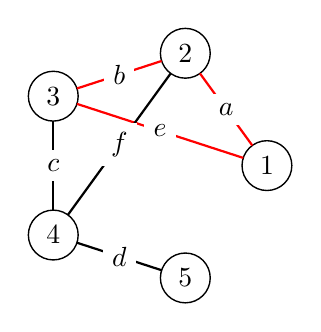
\begin{tikzpicture}
        %\GraphInit[vstyle=Welsh]
        \SetGraphUnit{1.5}
        \Vertices{circle}{1, 2, 3, 4, 5}
        \Edges[label=$a$, color=red](1, 2)
        \Edges[label=$b$, color=red](2, 3)
        \Edges[label=$c$](3, 4)
        \Edges[label=$d$](4, 5)
        \Edges[label=$e$, color=red](1, 3)
        \Edges[label=$f$](2, 4)
    \end{tikzpicture}
\end{center}
}
\only<3>{
\begin{center}
    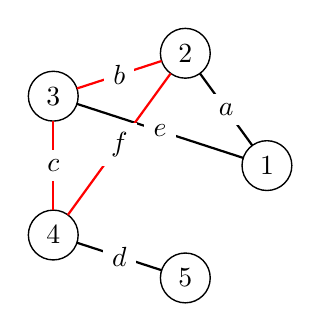
\begin{tikzpicture}
        %\GraphInit[vstyle=Welsh]
        \SetGraphUnit{1.5}
        \Vertices{circle}{1, 2, 3, 4, 5}
        \Edges[label=$a$](1, 2)
        \Edges[label=$b$, color=red](2, 3)
        \Edges[label=$c$, color=red](3, 4)
        \Edges[label=$d$](4, 5)
        \Edges[label=$e$](1, 3)
        \Edges[label=$f$, color=red](2, 4)
    \end{tikzpicture}
\end{center}
}
\end{frame}

\begin{frame}[t]
{Preliminaries}
Let $G = (V, E)$ be a graph.
\begin{itemize}
    \item Tree: connected graph without cycle
    \item<2-> Spanning tree
\end{itemize}

\only<3>{
\begin{center}
    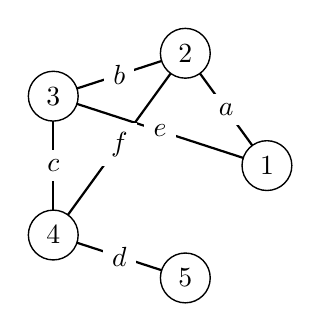
\begin{tikzpicture}
        %\GraphInit[vstyle=Welsh]
        \SetGraphUnit{1.5}
        \Vertices{circle}{1, 2, 3, 4, 5}
        \Edges[label=$a$](1, 2)
        \Edges[label=$b$](2, 3)
        \Edges[label=$c$](3, 4)
        \Edges[label=$d$](4, 5)
        \Edges[label=$e$](1, 3)
        \Edges[label=$f$](2, 4)
    \end{tikzpicture}
\end{center}
}
\only<4>{
\begin{center}
    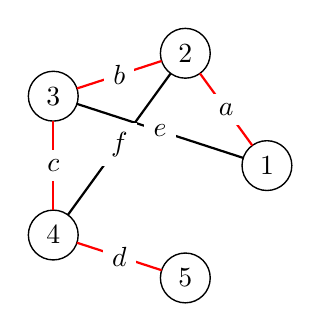
\begin{tikzpicture}
        %\GraphInit[vstyle=Welsh]
        \SetGraphUnit{1.5}
        \Vertices{circle}{1, 2, 3, 4, 5}
        \Edges[label=$a$, color=red](1, 2)
        \Edges[label=$b$, color=red](2, 3)
        \Edges[label=$c$, color=red](3, 4)
        \Edges[label=$d$, color=red](4, 5)
        \Edges[label=$e$](1, 3)
        \Edges[label=$f$](2, 4)
    \end{tikzpicture}
\end{center}
}
\only<5>{

\begin{center}
    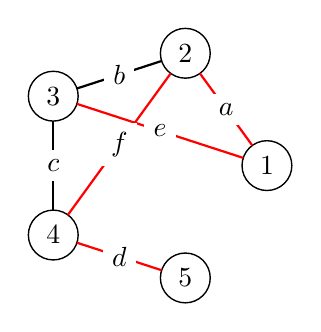
\begin{tikzpicture}
        %\GraphInit[vstyle=Welsh]
        \SetGraphUnit{1.5}
        \Vertices{circle}{1, 2, 3, 4, 5}
        \Edges[label=$a$, color=red](1, 2)
        \Edges[label=$b$](2, 3)
        \Edges[label=$c$](3, 4)
        \Edges[label=$d$, color=red](4, 5)
        \Edges[label=$e$, color=red](1, 3)
        \Edges[label=$f$, color=red](2, 4)
    \end{tikzpicture}
\end{center}
}
    
\end{frame}

\section{What is a matroid?}
\frame{\sectionpage}

\begin{frame}[t]
{Example from matrix}

Consider:
\begin{itemize}
    \item $ A = 
        \begin{bmatrix}
        1 & 0 & 0 & 1 \\
        0 & 3 & 0 & 3 \\
        2 & 4 & 2 & 6
        \end{bmatrix}$ over the field $\mathbb{R}$.
    \item $C = \{1, 2, 3, 4\}$ : the set of column vectors
\end{itemize}

\only<2->{
Then,
\begin{itemize}
    \item $\emptyset$, $\{1, 2\}$, $\{1, 2, 3\}$, $\{3, 4\}$, $\{2, 3\}$, $\cdots$: linearly independent
    \item $\{1, 2, 4\}$, $\{1, 2, 3, 4\}$, $\cdots$: linearly dependent
\end{itemize}
}

\only<3->{
There is a strange fact:
\begin{itemize}
    \item All the bases(=maximal independent sets) have the same size.
\end{itemize}
}

\end{frame}

\begin{frame}[t]
{Example from graph}
Let $G = (V, E)$ be a graph.
\only<2->{
\begin{center}
    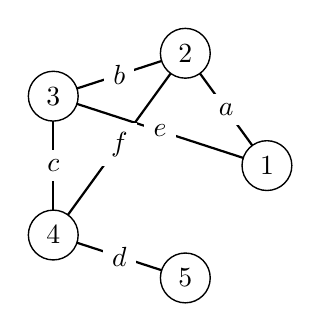
\begin{tikzpicture}
        %\GraphInit[vstyle=Welsh]
        \SetGraphUnit{1.5}
        \Vertices{circle}{1, 2, 3, 4, 5}
        \Edges[label=$a$](1, 2)
        \Edges[label=$b$](2, 3)
        \Edges[label=$c$](3, 4)
        \Edges[label=$d$](4, 5)
        \Edges[label=$e$](1, 3)
        \Edges[label=$f$](2, 4)
    \end{tikzpicture}
\end{center}
}
\only<2>{
\begin{itemize}
    \item $\{a\}, \{a, b\}, \{a, b, c\}, \{a, b, c, d\}, \{a, c, d, f\}$: acyclic
    \item $\{a, b, c, e\}$, $\{a, b, e\}$, $\{a, b, c, f\}$: contains cycle
\end{itemize}
}
\only<3>{
There is a strange fact:
\begin{itemize}
    \item All the maximal acyclic subset(i.e. spanning tree) of $E$ have the same size.
\end{itemize}
}
\end{frame}

\begin{frame}[t]
{What is a matroid?}

Can we find a common generalization of those examples?

\only<2->{
\begin{block}{Matroid [Whitney, 1935]}
A matroid is a pair $M = (S, \I)$ of a finite set $S$ and a set $\I \subseteq 2^S$ satisfying:
\begin{itemize}
    \item[(I1)] $\emptyset \in \I$
    \item[(I2)] If $X \subseteq Y$ and $Y \in \I$, then $X \in \I$
    \item[(I3)] If $X, Y \in\I$ and $|X| < |Y|$, then $X \cup \{e\} \in \I$ for some $e \in Y - X$. 
\end{itemize}
\end{block}
}
\only<3>{
(I3) looks somewhat similar to following theorem from linear algebra.
\begin{center}
    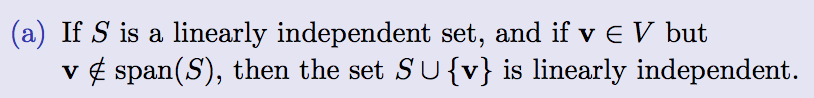
\includegraphics[width=\textwidth]{images/pmthm.png}
\end{center}
}
\only<4>{
We can easily obtain following property from (I3).
\begin{block}{Property}
All the maximal \emph{independent} set have the same size, and they are called the \emph{bases}. We denote the set of bases as $\B$.
\end{block}
}
\end{frame}

\begin{frame}[t]
{Example of matroids}

\begin{block}{Uniform matroids}
For $n \ge r \ge 0$, $U_{r, n}$ is a matroid on $[n] = \{1, 2, \cdots, n\}$ such that $X$ is independent if and only if $|X| \le r$.
\end{block}

\only<2->{
\begin{block}{Vector matroid}
For a matrix $A$ over the field $\F$, the \emph{vector matroid} $M[A]$ is the matroid on $C$, the column set of $A$, where $X \subseteq C$ is independent if and only if $A[X]$ is linearly independent.
\end{block}
}
\only<3>{
Note that:
\begin{itemize}
    \item If $ A = 
        \begin{bmatrix}
        1 & 0 & 0 & 1 \\
        0 & 3 & 0 & 3 \\
        2 & 4 & 2 & 4
        \end{bmatrix}$,
        then $A[\{1, 2, 4\}] = 
        \begin{bmatrix}
        1 & 0 & 1  \\
        0 & 3 & 3  \\
        2 & 4 & 4 
        \end{bmatrix}$
\end{itemize}
}
\only<4>{
    We can easily check that the base of $M[A]$ corresponds to the column base of $A$.
}

\only<5>{
\begin{block}{Cycle matroid}
For a graph $G = (V, E)$, the \emph{Cycle matroid} $M(G)$ is a matroid on $E$ s.t. $X \subseteq E$ is independent if $X$ contains no cycle.
\end{block}
}

\end{frame}

\begin{frame}[t]{Graph vs. Weighted Graph}

\only<1>{
Graph $G = (V, E)$
\begin{center}
    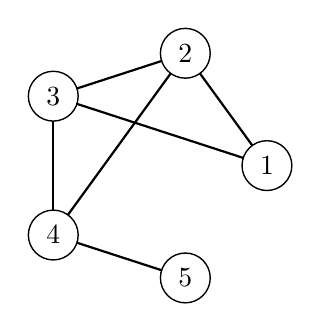
\begin{tikzpicture}
        %\GraphInit[vstyle=Welsh]
        \SetGraphUnit{1.5}
        \Vertices{circle}{1, 2, 3, 4, 5}
        \Edges[](1, 2)
        \Edges[](2, 3)
        \Edges[](3, 4)
        \Edges[](4, 5)
        \Edges[](1, 3)
        \Edges[](2, 4)
    \end{tikzpicture}
\end{center}
}
\only<2>{
Weighted graph $G = (V, E, {\color{red}w})$, $w : \alert{E} \to \mathbb{R}$
\begin{center}
    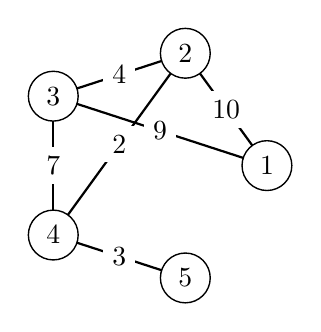
\begin{tikzpicture}
        %\GraphInit[vstyle=Welsh]
        \SetGraphUnit{1.5}
        \Vertices{circle}{1, 2, 3, 4, 5}
        \Edges[label=$10$](1, 2)
        \Edges[label=$4$](2, 3)
        \Edges[label=$7$](3, 4)
        \Edges[label=$3$](4, 5)
        \Edges[label=$9$](1, 3)
        \Edges[label=$2$](2, 4)
    \end{tikzpicture}
\end{center}
}
    
\end{frame}

\begin{frame}[t]{Weighted matroids}

\begin{block}{Weighted matroids}
\begin{itemize}
    \item $M = (S, \I, w)$ is a weighted matroid if $(S, \I)$ is a matroid and $w : S \to \mathbb{R}_{\ge 0}$
    \item<2-> For $A \subseteq S$, the \emph{weight} of $A$ is the sum of its elements, that is, $w(A) = \sum_{e \in A} w(e)$.
    \item<3-> $\I^\star := \{A \in \I : w(A) \text{ is maximum}\}$
    \item<4-> $\displaystyle w(\I^\star) := \max_{A \in \I} w(A)$
\end{itemize}
\end{block}
    
\end{frame}

\begin{frame}[t]{Example of weighted matroids}

Consider following graph:
\only<1>{
\begin{center}
    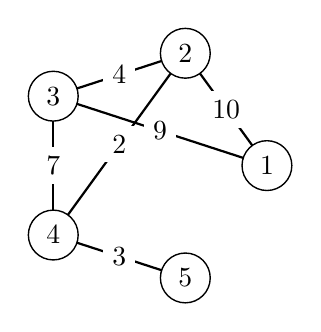
\begin{tikzpicture}
        %\GraphInit[vstyle=Welsh]
        \SetGraphUnit{1.5}
        \Vertices{circle}{1, 2, 3, 4, 5}
        \Edges[label=$10$](1, 2)
        \Edges[label=$4$](2, 3)
        \Edges[label=$7$](3, 4)
        \Edges[label=$3$](4, 5)
        \Edges[label=$9$](1, 3)
        \Edges[label=$2$](2, 4)
    \end{tikzpicture}
\end{center}
}
\only<2->{
\begin{center}
    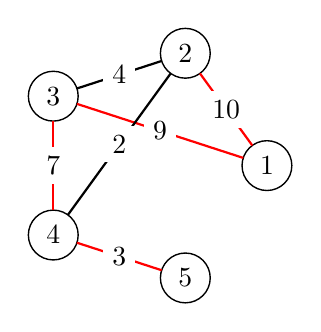
\begin{tikzpicture}
        %\GraphInit[vstyle=Welsh]
        \SetGraphUnit{1.5}
        \Vertices{circle}{1, 2, 3, 4, 5}
        \Edges[label=$10$, color=red](1, 2)
        \Edges[label=$4$](2, 3)
        \Edges[label=$7$, color=red](3, 4)
        \Edges[label=$3$, color=red](4, 5)
        \Edges[label=$9$, color=red](1, 3)
        \Edges[label=$2$](2, 4)
    \end{tikzpicture}
\end{center}
}
\begin{itemize}
    \item<2-> $\I^\star$ is the set of maximum-weight spanning trees
    \item<3-> $w(\I^\star)$ is the weight of maximum spanning tree
\end{itemize}
    
\end{frame}


\section{Greedy algorithms}
\frame{\sectionpage}

\begin{frame}[t]
{Spanning trees and greedy algorithms}

Recall the previous example.

\begin{center}
    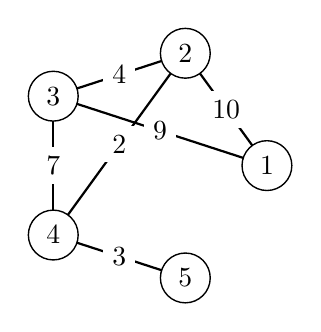
\begin{tikzpicture}
        %\GraphInit[vstyle=Welsh]
        \SetGraphUnit{1.5}
        \Vertices{circle}{1, 2, 3, 4, 5}
        \Edges[label=$10$](1, 2)
        \Edges[label=$4$](2, 3)
        \Edges[label=$7$](3, 4)
        \Edges[label=$3$](4, 5)
        \Edges[label=$9$](1, 3)
        \Edges[label=$2$](2, 4)
    \end{tikzpicture}
\end{center}

\begin{itemize}
    \item<2-> How can we find maximum/minimum weighted spanning trees?
\end{itemize}
    
\end{frame}

\begin{frame}[t]
{Spanning trees and greedy algorithms}
You might heard of it if you have taken CS300 (Introduction to Algorithms) or etc.
\only<2->{
\begin{block}{Kruskal's MST algorithm}
SpanningTree($G = (V, E, w)$)
\begin{itemize}
    \item<3-> $T := \emptyset$
    \item<4-> Sort $E = \{e_1, e_2, \cdots, e_n \}$ so that $w(e_1) \ge w(e_2) \ge \cdots w(e_n)$.
    \item<5-> for ($i:=1$ to $n$) do
    \begin{itemize}
        \item<6-> if $T \cup \{e_i\}$ contains no cycle
        \begin{itemize}
            \item<7-> $T := T \cup \{e_i\}$
        \end{itemize}
    \end{itemize}
    \item<8-> return $T$
\end{itemize}
\end{block}
}
%\only<9>{
%Above algorithm finds an element of $\I^\star$ of a cycle matroid. Can we generalize it more general?
%}
\end{frame}

\begin{frame}[t]
{Kruskal's MST algorithm}

Demo of Kruskal's algorithm
\only<1>{
\begin{center}
    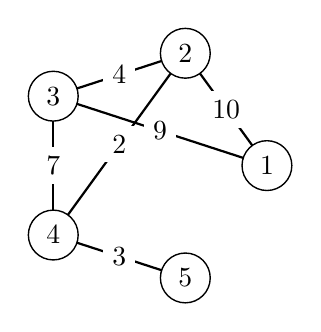
\begin{tikzpicture}
        %\GraphInit[vstyle=Welsh]
        \SetGraphUnit{1.5}
        \Vertices{circle}{1, 2, 3, 4, 5}
        \Edges[label=$10$](1, 2)
        \Edges[label=$4$](2, 3)
        \Edges[label=$7$](3, 4)
        \Edges[label=$3$](4, 5)
        \Edges[label=$9$](1, 3)
        \Edges[label=$2$](2, 4)
    \end{tikzpicture}
\end{center}
}
\only<2>{
\begin{center}
    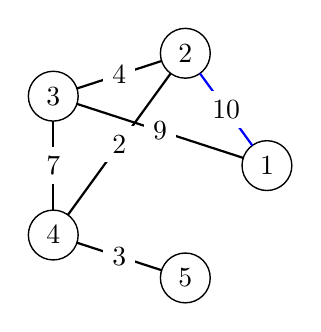
\begin{tikzpicture}
        %\GraphInit[vstyle=Welsh]
        \SetGraphUnit{1.5}
        \Vertices{circle}{1, 2, 3, 4, 5}
        \Edges[label=$10$, color=blue](1, 2)
        \Edges[label=$4$](2, 3)
        \Edges[label=$7$](3, 4)
        \Edges[label=$3$](4, 5)
        \Edges[label=$9$](1, 3)
        \Edges[label=$2$](2, 4)
    \end{tikzpicture}
\end{center}
}

\only<3>{
\begin{center}
    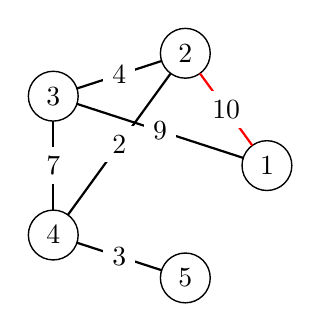
\begin{tikzpicture}
        %\GraphInit[vstyle=Welsh]
        \SetGraphUnit{1.5}
        \Vertices{circle}{1, 2, 3, 4, 5}
        \Edges[label=$10$, color=red](1, 2)
        \Edges[label=$4$](2, 3)
        \Edges[label=$7$](3, 4)
        \Edges[label=$3$](4, 5)
        \Edges[label=$9$](1, 3)
        \Edges[label=$2$](2, 4)
    \end{tikzpicture}
\end{center}
}
\only<4>{
\begin{center}
    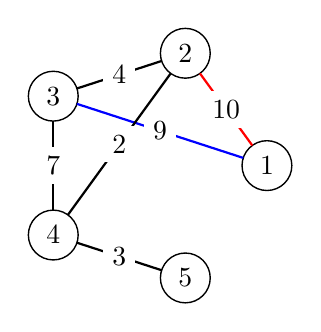
\begin{tikzpicture}
        %\GraphInit[vstyle=Welsh]
        \SetGraphUnit{1.5}
        \Vertices{circle}{1, 2, 3, 4, 5}
        \Edges[label=$10$, color=red](1, 2)
        \Edges[label=$4$](2, 3)
        \Edges[label=$7$](3, 4)
        \Edges[label=$3$](4, 5)
        \Edges[label=$9$, color=blue](1, 3)
        \Edges[label=$2$](2, 4)
    \end{tikzpicture}
\end{center}
}
\only<5>{
\begin{center}
    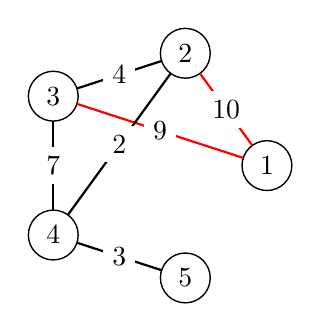
\begin{tikzpicture}
        %\GraphInit[vstyle=Welsh]
        \SetGraphUnit{1.5}
        \Vertices{circle}{1, 2, 3, 4, 5}
        \Edges[label=$10$, color=red](1, 2)
        \Edges[label=$4$](2, 3)
        \Edges[label=$7$](3, 4)
        \Edges[label=$3$](4, 5)
        \Edges[label=$9$, color=red](1, 3)
        \Edges[label=$2$](2, 4)
    \end{tikzpicture}
\end{center}
}
\only<6>{
\begin{center}
    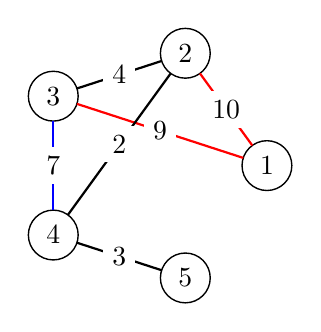
\begin{tikzpicture}
        %\GraphInit[vstyle=Welsh]
        \SetGraphUnit{1.5}
        \Vertices{circle}{1, 2, 3, 4, 5}
        \Edges[label=$10$, color=red](1, 2)
        \Edges[label=$4$](2, 3)
        \Edges[label=$7$, color=blue](3, 4)
        \Edges[label=$3$](4, 5)
        \Edges[label=$9$, color=red](1, 3)
        \Edges[label=$2$](2, 4)
    \end{tikzpicture}
\end{center}
}
\only<7>{
\begin{center}
    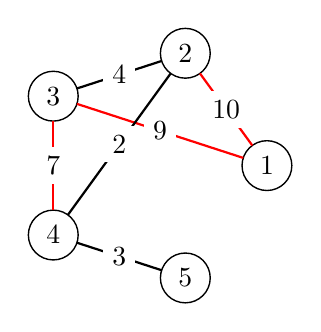
\begin{tikzpicture}
        %\GraphInit[vstyle=Welsh]
        \SetGraphUnit{1.5}
        \Vertices{circle}{1, 2, 3, 4, 5}
        \Edges[label=$10$, color=red](1, 2)
        \Edges[label=$4$](2, 3)
        \Edges[label=$7$, color=red](3, 4)
        \Edges[label=$3$](4, 5)
        \Edges[label=$9$, color=red](1, 3)
        \Edges[label=$2$](2, 4)
    \end{tikzpicture}
\end{center}
}
\only<8>{
\begin{center}
    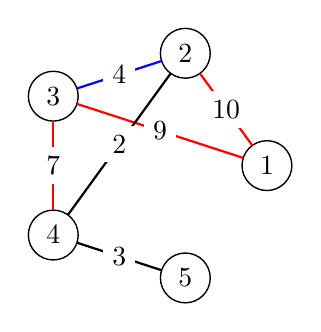
\begin{tikzpicture}
        %\GraphInit[vstyle=Welsh]
        \SetGraphUnit{1.5}
        \Vertices{circle}{1, 2, 3, 4, 5}
        \Edges[label=$10$, color=red](1, 2)
        \Edges[label=$4$, color=blue](2, 3)
        \Edges[label=$7$,, color=red](3, 4)
        \Edges[label=$3$](4, 5)
        \Edges[label=$9$, color=red](1, 3)
        \Edges[label=$2$](2, 4)
    \end{tikzpicture}
\end{center}
}
\only<9>{
\begin{center}
    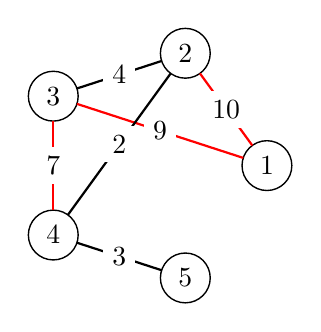
\begin{tikzpicture}
        %\GraphInit[vstyle=Welsh]
        \SetGraphUnit{1.5}
        \Vertices{circle}{1, 2, 3, 4, 5}
        \Edges[label=$10$, color=red](1, 2)
        \Edges[label=$4$](2, 3)
        \Edges[label=$7$, color=red](3, 4)
        \Edges[label=$3$](4, 5)
        \Edges[label=$9$, color=red](1, 3)
        \Edges[label=$2$](2, 4)
    \end{tikzpicture}
\end{center}
}
\only<10>{
\begin{center}
    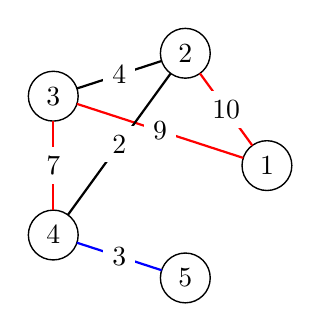
\begin{tikzpicture}
        %\GraphInit[vstyle=Welsh]
        \SetGraphUnit{1.5}
        \Vertices{circle}{1, 2, 3, 4, 5}
        \Edges[label=$10$, color=red](1, 2)
        \Edges[label=$4$](2, 3)
        \Edges[label=$7$, color=red](3, 4)
        \Edges[label=$3$, color=blue](4, 5)
        \Edges[label=$9$, color=red](1, 3)
        \Edges[label=$2$](2, 4)
    \end{tikzpicture}
\end{center}
}
\only<11>{
\begin{center}
    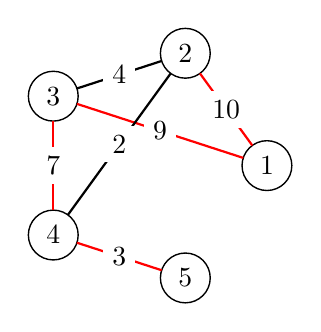
\begin{tikzpicture}
        %\GraphInit[vstyle=Welsh]
        \SetGraphUnit{1.5}
        \Vertices{circle}{1, 2, 3, 4, 5}
        \Edges[label=$10$, color=red](1, 2)
        \Edges[label=$4$](2, 3)
        \Edges[label=$7$, color=red](3, 4)
        \Edges[label=$3$, color=red](4, 5)
        \Edges[label=$9$, color=red](1, 3)
        \Edges[label=$2$](2, 4)
    \end{tikzpicture}
\end{center}
}
\only<12>{
\begin{center}
    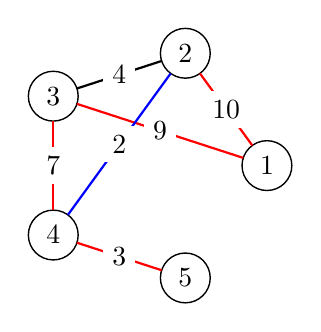
\begin{tikzpicture}
        %\GraphInit[vstyle=Welsh]
        \SetGraphUnit{1.5}
        \Vertices{circle}{1, 2, 3, 4, 5}
        \Edges[label=$10$, color=red](1, 2)
        \Edges[label=$4$](2, 3)
        \Edges[label=$7$, color=red](3, 4)
        \Edges[label=$3$, color=red](4, 5)
        \Edges[label=$9$, color=red](1, 3)
        \Edges[label=$2$, color=blue](2, 4)
    \end{tikzpicture}
\end{center}
}
\only<13>{
\begin{center}
    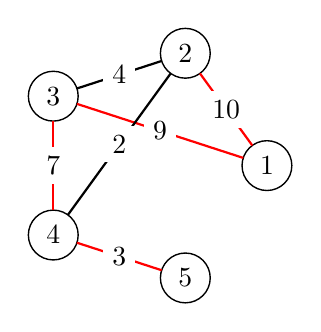
\begin{tikzpicture}
        %\GraphInit[vstyle=Welsh]
        \SetGraphUnit{1.5}
        \Vertices{circle}{1, 2, 3, 4, 5}
        \Edges[label=$10$, color=red](1, 2)
        \Edges[label=$4$](2, 3)
        \Edges[label=$7$, color=red](3, 4)
        \Edges[label=$3$, color=red](4, 5)
        \Edges[label=$9$, color=red](1, 3)
        \Edges[label=$2$](2, 4)
    \end{tikzpicture}
\end{center}
}
    
\end{frame}

\begin{frame}[t]
{Spanning trees and greedy algorithms}
You might heard of it if you have taken CS300 (Introduction to Algorithms) or etc.
\begin{block}{Kruskal's MST algorithm}
SpanningTree($G = (V, E, w)$)
\begin{itemize}
    \item $T := \emptyset$
    \item Sort $E = \{e_1, e_2, \cdots, e_n \}$ so that $w(e_1) \ge w(e_2) \ge \cdots w(e_n)$.
    \item for ($i:=1$ to $n$) do
    \begin{itemize}
        \item if $T \cup \{e_i\}$ contains no cycle
        \begin{itemize}
            \item $T := T \cup \{e_i\}$
        \end{itemize}
    \end{itemize}
    \item return $T$
\end{itemize}
\end{block}

\only<2>{
Above algorithm finds an element of $\I^\star$ of a cycle matroid. Can we generalize it more general?
}
\end{frame}

\begin{frame}[t]
{Generalized algorithm}
\only<2->{
\begin{block}{Generalized greedy algorithm}
Greedy($M = (S, \I, w)$) \texttt{// Goal: to find some $A \in \I^\star$}
\begin{itemize}
    \item<3-> $A := \emptyset$
    \item<4-> Sort $S = \{x_1, x_2, \cdots, x_n\}$ so that $w(x_1) \ge w(x_2) \ge \cdots \ge w(x_n)$.
    \item<5-> for ($i:=1$ to $n$) do
    \begin{itemize}
        \item<6-> if $A \cup \{x_i\} \in \I$
        \begin{itemize}
            \item<7-> $A := A \cup \{x_i\}$
        \end{itemize}
    \end{itemize}
    \item<8-> return $A$ \texttt{// $A \in \I^\star$?}
\end{itemize}
\end{block}
}
\only<9->{
So, is this algorithm \emph{actually} works (correctly) for any matroid?
}
\begin{itemize}
    \item<10> Let's prove it!
\end{itemize}
\end{frame}

\begin{frame}[t]
{Correctness Proof}
\only<1-2>{For sake of convenience, sort $S = \{x_1, \cdots, x_n\}$ so that $w(x_1) \ge \cdots \ge w(x_n)$.}
\only<2->{
\begin{block}{Lemma 1}
Let $\{x_i\}$ be the \emph{first} element that $\{x_i\} \in \I$. Then, some $A \in \I^\star$ contains $x_i$.
\end{block}
}
\begin{itemize}
    \item<3-> To prove it, take any $B \in \I^\star$.
    \item<4-> If $x_i \in B$, done. Otherwise, construct $A$ inductively.
\end{itemize}
\only<5->{
\begin{block}{Algorithm to construct $A$}
\begin{itemize}
    \item $A := \{x_i\}$ initially
    \item while ($|A| < |B|$) do
    \begin{itemize}
        \item Take $x' \in B-A$ such that $A \cup \{x'\} \in \I$ \texttt{//(I3)}
        \item $A := A \cup \{x'\}$
    \end{itemize}
\end{itemize}
\end{block}
}
\only<6>{
\begin{itemize}
    \item Then, $A = B \cup \{x_i\} - \{x_j\}$ for some $j > i$ so that
    $$ w(I^\star) \ge w(A) = w(B) - w(x_j) + w(x_i) \ge w(B) = w(I^\star). $$
\end{itemize}
}
\end{frame}

\begin{frame}[t]
{Correctness Proof}

\begin{block}{Lemma 2}
For $x \in S$, if $\{x \} \not \in \I$, then no element of $\I$ contains $x$.
\end{block}

\only<2->{
Its proof is clear from (I2).
}
    
\end{frame}

\begin{frame}[t]
{Correctness Proof}

\begin{block}{Definition 1}
For a weighted matroid $M = (S, \I, w)$ and $x \in S$, we define new weighted matroid $M_x = (S_x, \I_x, w_x)$ as:
\begin{itemize}
    \item $S_x = \{y \in S - \{x\} : \{x, y\} \in \I\}$
    \item $\I_x = \{B \subseteq S- \{x\} : B \cup \{x\} \in \I\}$
    \item $w_x = w|_{S_x}$
\end{itemize}
if $S_x \neq \emptyset$, it is \emph{acutally} a matroid.
\end{block}
\only<2->{
\begin{block}{Lemma 3 - Optimal substructure property}
Let $M = (S, \I, w)$ be a weighted matroid and suppose $x \in S$ satisfies:
\begin{itemize}
    \item $x$ is contained by some element of $\I^\star$.
\end{itemize}
Then, for each $B \in \I_x^\star$, $B \cup \{x\} \in \I^\star$.
\end{block}
}

\end{frame}

\begin{frame}[t]
{Correctness Proof}
\begin{block}{Lemma 3 - Optimal substructure property}
Let $M = (S, \I, w)$ be a weighted matroid and suppose $x \in S$ satisfies:
\begin{itemize}
    \item $x$ is contained by some element of $\I^\star$.
\end{itemize}
Then, for each $B \in \I_x^\star$, $B \cup \{x\} \in \I^\star$.
\end{block}

\begin{itemize}
    \item<2-> Show $w(\I^\star) = w(\I_x^\star) + w(x)$.
    \item<3-> So, for $B \in \I_x^\star$, $w(B \cup \{x\}) = w(B) + w(x) = w(\I_x^\star) + w(x) = w(\I^\star)$.
\end{itemize}

\only<4>{Combining those things all together, we can show the algorithm works correctly.}
\end{frame}

\begin{frame}[t]
{Generalized algorithm}
We have shown that below algorithm works correctly for every (weighted) matroid.
\only<2->{
\begin{block}{Generalized greedy algorithm}
Greedy($M = (S, \I, w)$) \texttt{// Goal: to find some $A \in \I^\star$}
\begin{itemize}
    \item $A := \emptyset$
    \item Sort $S = \{x_1, x_2, \cdots, x_n\}$ so that $w(x_1) \ge w(x_2) \ge \cdots \ge w(x_n)$.
    \item for ($i:=1$ to $n$) do
    \begin{itemize}
        \item if $A \cup \{x_i\} \in \I$ //$(\star)$
        \begin{itemize}
            \item $A := A \cup \{x_i\}$
        \end{itemize}
    \end{itemize}
    \item return $A$ \texttt{// $A \in \I^\star$}
\end{itemize}
\end{block}
}
\begin{itemize}
    \item<3> Furthermore, it is efficient since it only takes $\mathcal{O}(n \log n + nf(n))$ time where $f(n)$ is running time of $(\star)$.
\end{itemize}
\end{frame}

\begin{frame}[t]
{Generalized algorithm}
We have shown that below algorithm works correctly for every (weighted) matroid.

\begin{block}{Generalized greedy algorithm}
Greedy($M = (S, \I, w)$) \texttt{// Goal: to find some $A \in \I^\star$}
\begin{itemize}
    \item $A := \emptyset$
    \item Sort $S = \{x_1, x_2, \cdots, x_n\}$ so that $w(x_1) \ge w(x_2) \ge \cdots \ge w(x_n)$.
    \item for ($i:=1$ to $n$) do
    \begin{itemize}
        \item if $A \cup \{x_i\} \in \I$
        \begin{itemize}
            \item $A := A \cup \{x_i\}$
        \end{itemize}
    \end{itemize}
    \item return $A$ \texttt{// $A \in \I^\star$}
\end{itemize}
\end{block}

\begin{itemize}
    \item Q. Can we use matroid to formulate problems that \emph{generic greedy algorithm} works correctly?
\end{itemize}
\end{frame}

\begin{frame}[t]
{Defining matroid from greedy algorithms}
\begin{block}{Theorem}
Suppose that we are given a finite set $S$ and $\I \subseteq 2^S$ satisfying (I1) \only<1>{\underline{$\emptyset \in \I$} }and (I2)\only<1>{ \underline{Subset of independent set is independent}}.
If (G) holds, $M = (S, \I)$ is a matroid.
\begin{itemize}
    \item[(G)] Generic greedy algorithm works correctly for every $w : S \to \mathbb{R}$.
\end{itemize}
\end{block}
\begin{itemize}
    \item<2-> Suppose that (I3) does not holds for some $X, Y \in \I$.
    \only<3>{
    \begin{itemize}
        \item<3> That is, $X \cup \{e\} \not \in \I$ for every $e \in Y-X$.
    \end{itemize}
    }
    \item<4-> For sufficient $0 < \epsilon < (|Y|-|X|)/|X-Y|$, define
    $
    w(x) =
    \begin{cases}
    1 + \epsilon & \text{if } x \in X \\
    1 & \text{if } x \in Y - X \\
    0 & \text{otherwise}
    \end{cases}.
    $
    \item<5-> Then, $X'$, result of greedy algorithm contains $X$ so that $|Y| + \epsilon |X \cap Y| = w(Y) \le w(X') = (1+\epsilon)|X|$, which implies $\epsilon |X-Y| \ge |Y|-|X|$.
\end{itemize}
\end{frame}

\begin{frame}[t]
{Results}
Interestingly, although matroid is the concept that defines (linear) \emph{independence} combinatorially, we checked that it also characterizes generic greedy algorithm.
\begin{block}{Generalized greedy algorithm}
Greedy($M = (S, \I, w)$) \texttt{// Goal: to find some $A \in \I^\star$}
\begin{itemize}
    \item $A := \emptyset$
    \item Sort $S = \{x_1, x_2, \cdots, x_n\}$ so that $w(x_1) \ge w(x_2) \ge \cdots \ge w(x_n)$.
    \item for ($i:=1$ to $n$) do
    \begin{itemize}
        \item if $A \cup \{x_i\} \in \I$
        \begin{itemize}
            \item $A := A \cup \{x_i\}$
        \end{itemize}
    \end{itemize}
    \item return $A$ \texttt{// $A \in \I^\star$}
\end{itemize}
\end{block}
\end{frame}\begin{frame}[t]
{References}
\begin{itemize}
    \item James Oxley, \emph{Matroid theory}, second ed., Oxford, 2011
    \item James Oxley, \emph{What is a matroid?}, \texttt{\url{https://www.math.lsu.edu/~oxley/survey4.pdf}}
\end{itemize}
\end{frame}
\end{document}
